\documentclass[10pt,twocolumn,letterpaper]{article}

\usepackage{cvpr}
\usepackage{times}
\usepackage{epsfig}
\usepackage{graphicx}
\usepackage{amsmath}
\usepackage{amssymb}

% Include other packages here, before hyperref.

% If you comment hyperref and then uncomment it, you should delete
% egpaper.aux before re-running latex.  (Or just hit 'q' on the first latex
% run, let it finish, and you should be clear).
\usepackage[breaklinks=true,bookmarks=false]{hyperref}

\cvprfinalcopy % *** Uncomment this line for the final submission

\def\cvprPaperID{****} % *** Enter the CVPR Paper ID here
\def\httilde{\mbox{\tt\raisebox{-.5ex}{\symbol{126}}}}

% Pages are numbered in submission mode, and unnumbered in camera-ready
%\ifcvprfinal\pagestyle{empty}\fi
% \setcounter{page}{4321}
\begin{document}
	
	%%%%%%%%% TITLE
	\title{Mask inpainting with a GAN network}
	
	\author{Luca Lumetti\\
		{\tt\small 244577@studenti.unimore.it}
		% For a paper whose authors are all at the same institution,
		% omit the following lines up until the closing ``}''.
		% Additional authors and addresses can be added with ``\and'',
		% just like the second author.
		% To save space, use either the email address or home page, not both
		\and
		Federico Silvestri\\
		{\tt\small 243938@studenti.unimore.it}
		\and
		Matteo Di Bartolomeo\\
		{\tt\small 241469@studenti.unimore.it}
	}
	
	\maketitle
	%\thispagestyle{empty}
	
	%%%%%%%%% ABSTRACT
	\begin{abstract}
		Our project aims to remove a face mask over a person’s face, by reconstructing
		the covered part of the face. To have a more precise reconstruction of the
		missing parts (mouth and nose) behind the mask, we plan to use a second photo
		of the same person without the mask as a reference during the facial
		reconstruction process. There are no constraints on the quality of the
		reference photo, for instance the face can be taken from a different point of
		view than the first one. To sum up, given as input an image containing a
		person’s face partially covered by a medical mask and another photo of the
		same person without any occlusions, the output will be the first image with
		the mask-covered parts, mouth and nose, reconstructed. Future development
		could lead to generalizing the occlusion caused by the mask to any type of
		occlusion possible.
	\end{abstract}
	
	%%%%%%%%% BODY TEXT
	\section{Mask Segmentation}
	We made use of MediaPipe's FaceMesh \cite{DBLP:journals/corr/abs-1907-06724}
	library to find facial landmarks over the face covered with the surgical mask
	and the reference photo. Facial landmarks are important to have an initial
	approximation of the region where to search the surgical mask and to warp the
	reference photo over the first one. To perform the segmentation of the mask we
	apply a k-means with k=3 over the polygon we created using face landmarks and
	pick the bigger region between the 3.  The k has been choosen to be 3 as in the
	polygonal region we expect to find the mask, the background and the skin of the
	person's face. In the end, a binary image is created, with a 1 where the mask is
	present and 0 elsewhere, while in the original image, the mask area is filled
	with 0s.
	
	\section{Warping the reference photo}
	The objective of the reference photo is to guide the network to a more loyal
	reconstruction. As we allow the reference to have [avere un'angolazione diversa
	da quella frontale], we apply a thin-plate spline transformation to make it frontal
	[meh che traduzione brutta]. We use 30 specific landmarks as parameters as using
	more parameters lead to distortion given by the error in the landmarks detection
	and less lead to an imperfect warping. The same polygon region of Mask
	Segmentation is cut from the reference photo, the by applying the TPS is sticked
	to to main photo leading to a (partial) reconstruction.
	
	\section{Image inpainting}
	
	Image inpainting (a.k.a. image completion) is the task to fill a missing region
	in an image by predicting the value of the missing pixels in order to have a
	realistic image which is semantically close to the original one and visually correct.
	There are two different approches to achieve this task:
	\begin{enumerate}
		\item
		Low-level feature patch-matching which does not work pretty well with non-stationary use-cases (e.g. faces, objects or complicate scenes);
		\item
		Feed-forward models with deep convolutional networks which overcome the problem of prevoious case exploiting semantics learned on large scale dataset.
	\end{enumerate}
	\section{Our approach}
	We decided to follow the latter one designing a coarse-to-fine Generative Adversarial Network (GAN) characterized by:
	\begin{itemize}
		\item
		Generator:
		\begin{itemize}
			\item 
			Coarse network whose aim is to provide a rough estimation of missing pixels;
			\item
			Refinement network which takes the output of the previous network as input and takes care of its detailed decoration.
		\end{itemize}
		\item
		Discriminator which is responsible of distinguishing real samples from the one created by the generator.
	\end{itemize}
	The input of the network is a preprocessed RGB image so that its values are in range \([-1,+1]\).
	We provided different methods to initialize the strating values of the network weights, such as normal, Xavier, orthogonal and, the default one, Kaiming.
	\\
	We went for Adam as the generator and discriminator optimizer using a \(0.5\) momentum and different learning rates, respectively \(0.0001\) and \(0.0004\) for the first 10 epochs and then they will linearly decrease.
	%-------------------------------------------------------------------------
	\subsection{Network learning}
	Out function loss is the sum of five different loss fucntions:
	\begin{equation}
		\mathcal{L}_{tot} = \mathcal{L}_{gen} + \mathcal{L}_{recon} + \mathcal{L}_{tv} + \lambda_{perc} \cdot \mathcal{L}_{perc} + \lambda_{style} \cdot \mathcal{L}_{style}
	\end{equation}
	\textbf{Adversarial Loss.} It is the mean error calculated on the bad predictions of the discriminator
	\\
	\textbf{Reconstruction Loss.} It is the weighted sum of the outputs of the coarse and refinement networks, the calculated mask and the original input image.
	\\
	\textbf{Total variation (TV) Loss.} It is responsible of the regularization of the image to improve the smoothness of the output image.
	\\
	\textbf{Perceptual Loss.} It represents the L1-norm distance between high-level feature representations in 5 different convolutive layers. Its weight is set to \(0.05\).
	\\
	\textbf{Style Loss.}Using the same 5 levels of the previous loss, it is the sum of the distances of the auto-correlation matrixes between the output and the ground truth multiplied by a factor that depends on the size and number of the activation maps in those layers. Its weigth is set to \(40\).
	\\
	\subsection{Datasets}
	GAN networks are data-hungry and needs a lot of diverse training examples in
	order to generate quality images, for this reason we used the FFHQ 1024x1024
	images \cite{karras2019style}, rescaled to 256x256, during training.  In other GAN inpainting
	architectures, the mask region to reconstruct is usually calcuated during the
	training in a randomized way.  We do not have this randomization process, so for
	each image of FFHQ we precalculated the face region where the mask is weared
	using facial landmarks.  For testing we used CelebA256.
	
	\subsection{Architecture}
	Our architecture is highly inspired by Free Form Image Inpainting with Gated Convolution \cite{yu2019free} and DeepGIN \cite{li2020deepgin}.
	Our net is composed of two generators: Coarse Network and Refine Network.
	Both using Spatial Pyramid Dilation(SPD) that is a modified version of ResNet block. This layer is composed of different convolutional blocks with different dilation, and the output of these blocks is concatenated together.
	\begin{figure}[t]
		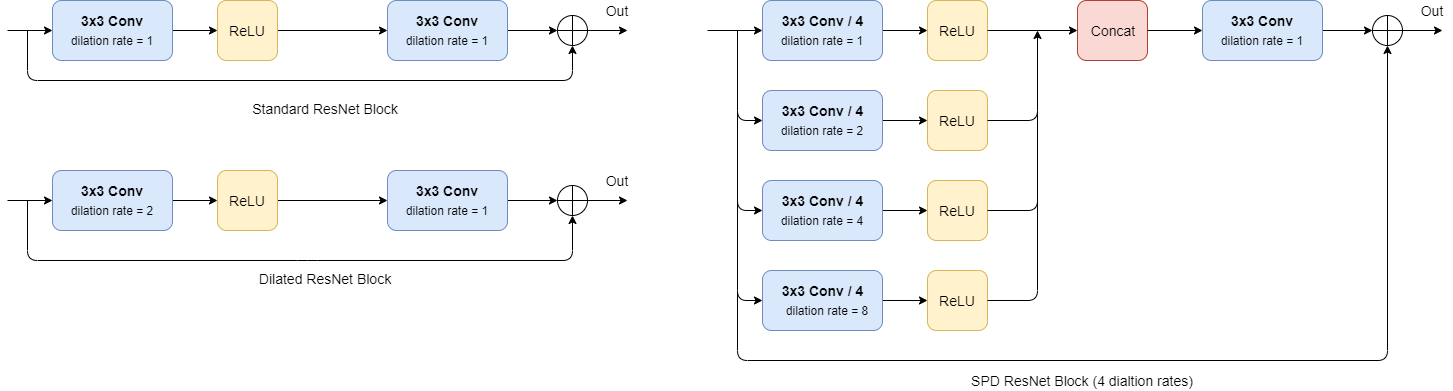
\includegraphics[width=1\linewidth]{img/ResNetSPD.png}
		\label{fig:long}
		\label{fig:onecol}
	\end{figure}
	\subsubsection{Coarse Network}
	In this stage we decided to use the gated convolution so that the generator is able to learn a dynamic feature selection mechanism for each channel and for each spatial location. The feature selection mechanism takes into account not only the background and the mask given in input, but also the semantic segmentation in some channels.
	Furthermore using gated convolutive layers we can avoid the inner drawbacks of vanilla and partial convolution. In fact taking a look to the vanilla convolution formula:
	\begin{equation}
		O_{y,x} = \sum_{i=-k'_h}^{k'_h}\sum_{j=-k'_w}^{k'_w} W_{k'_h + i, k'_w + j} \cdot I_{y + i, x + j}
	\end{equation}
	where \(O_{y,x}\) is the output, \(x,y\) represent x-axis and y-axis of the output map, \(k_h\) and \(k_w\) is the kernel size, \(k'_h = \frac{k_h - 1}{2}\),\(k'_w = \frac{k_w - 1}{2}\), \(W \in \mathbb{R}^{k_h \times k_w \times C' \times C}\) represents the convolutional filters and \(I_{y + i, x + j}\) is the input image, we can notice that it considers all pixels valid and it is applied to the entire input image. This cause color discrepancy and blurriness in final output image.
	\\
	In partial convolution, thanks to a masking and re-normalization step, the operation depends only on valid pixels:
	\begin{equation}
		O_{y,x} = \begin{cases}
			\sum \sum W \cdot (I \odot \frac{M}{sum(M)}), & \text{if sum(M) \(>\) 0} \\ 0 & \text{otherwise}
		\end{cases}
	\end{equation}
	
	\(M\) is the binary mask where a pixel with a value of 1 is considered valid and invalid with a value of 0 and \(\odot\) is the element-wise multiplication.
	There is a mask-update step based on the rule: \(m'_{y,x} = 1, iff sum(M) > 0\)
	\\
	This operation, however, has some problems:
	\begin{itemize}
		\item 
		It will set to one a pixel in next layer no matter the number of 1-value-pixels covered by the filter range in the previous layer;
		\item
		Invalid pixels will progressively fade out from the mask going deeper in the network layers;
		\item
		All channel in each layer shares the same mask limiting the flexibity of the model.
	\end{itemize}
	Gated convolution, instead, is based on the following formula:
	\begin{gather}
		Gating_{y,x} = \sum \sum W_g \cdot I \\
		Feature_{y,x} = \sum \sum W_f \cdot I \\
		O_{y,x} = \phi (Feature_{y,x}) \odot \sigma (Gating_{y,x})
	\end{gather}
	where there is sigmoid function \(\sigma\) to have the output in the range \([0,1]\), while \(\phi\) represents an activation function such ReLU, ELU and LeakyReLu (we used the latter). \(W_g\) and \(W_f\) are two different convolutional layers.
	\\
	As said before the benefits of using this operation is that the network is able to learn a mechanism to select feature dynamically for each channel and each spatial location considering also the semantic segmentation in some channels.
	\\
	As shown in \textbf{[Inserire riferimento alla figura]} the coarse net is charaterized by an initial downsampling phase, followed by a convolutional one and at the end there is and upsampling phase using the dilated gated convolution that could be seen as a gated convolution operation preceded by a resize operation. The output of the coarse net will pass through an activation function (we chose a \(\tanh\)) and the result will be given as input to the refinement network.
	\subsubsection{Refine Network}
	The second generator take the output of the coarse net and the mask and it's useful for refinement the image.
	In this stage there are 4 ResNet blocks with different dilation and some gated convolutional layers. in this manner, we can reduce the dimensions of the input and take a bigger receptive field. Another useful feature that is implemented in this net is the Multi Scale Self Attention (MSSA). The MSSA using the self-similarity between different layers and it's helpful to have a better coherence in the final image. We are control the self-similarity with three different scale: 16x16, 32x32, 64x64.
	
	
	\subsection{Results}
	PARTE METRICHE
	
	%------------------------------------------------------------------------
	
	{\small
		\bibliographystyle{plain}
		\bibliography{cvproject}
	}
	
\end{document}
